\subsection{Climate and Production}

\subsubsection{Climate Change Trend}
\begin{figure}[H]
    \centering
    \caption{Average Temperature since 1990 to 2021} 
    \label{fig:trend_avg_temp}
    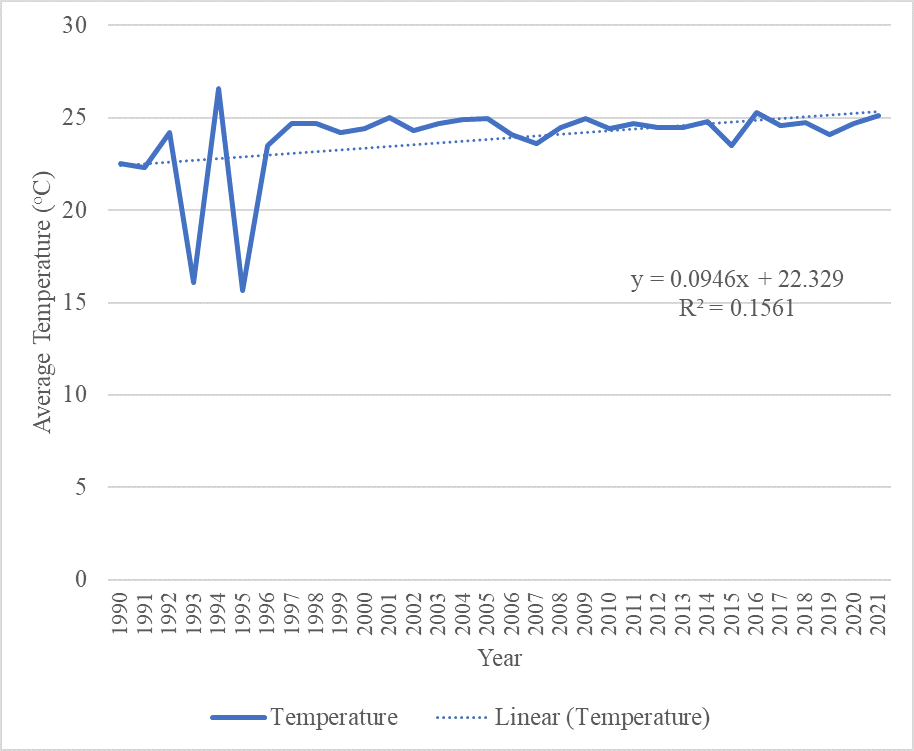
\includegraphics[width=0.9\textwidth]{images/trend_avg_temp.png}
\end{figure}

As shown in Figure~\ref{fig:trend_avg_temp}, the results indicate that between 1990 and 2020, the average temperature showed a minor positive trend, averaging 0.0946 degrees Celsius each year, with 15.61\% of the variability explained by the linear trend \( y = 0.0946x + 22.329 \). The positive trend might be due to global warming. The temperature increase could have a significant impact on crop production, as it may affect crop growth, development, and yield. The temperature increase could also lead to changes in the distribution of pests and diseases, which could further affect crop yield.

\begin{figure}[H]
    \centering
    \caption{Average Sunshine Hour since 1990 to 2021} 
    \label{fig:trend_avg_sunshine_hour}
    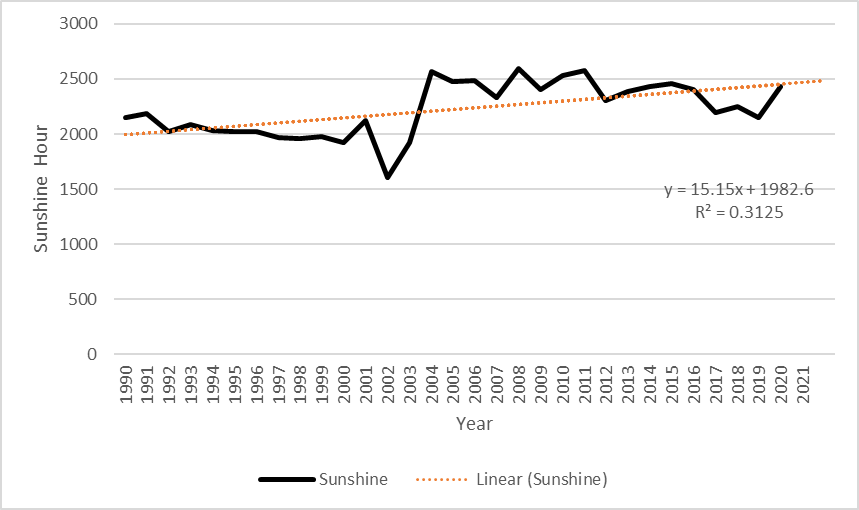
\includegraphics[width=0.9\textwidth]{images/trend_avg_sunshine_hour.png}
\end{figure}

The average sunlight hours from 1990 to 2020 showed a positive slope of 15.15 hours/year with an intercept of 1982.6 in the linear trend analysis. This indicated an overall rise in sunshine hours, and the trend's R-squared value of 0.3125 indicates that it accounts for 31.25\% of the variability (Figure~\ref{fig:trend_avg_sunshine_hour}). The increase in sunlight hours that Banke experienced between 1990 and 2020 might had been caused by variations in the weather, patterns of land use, and climate variability, all of which might had been impacted by local and global climate change.


\begin{figure}[H]
    \centering
    \caption{Accumulated Rainfall since 1990 to 2021} 
    \label{fig:trend_accumulated_rainfall}
    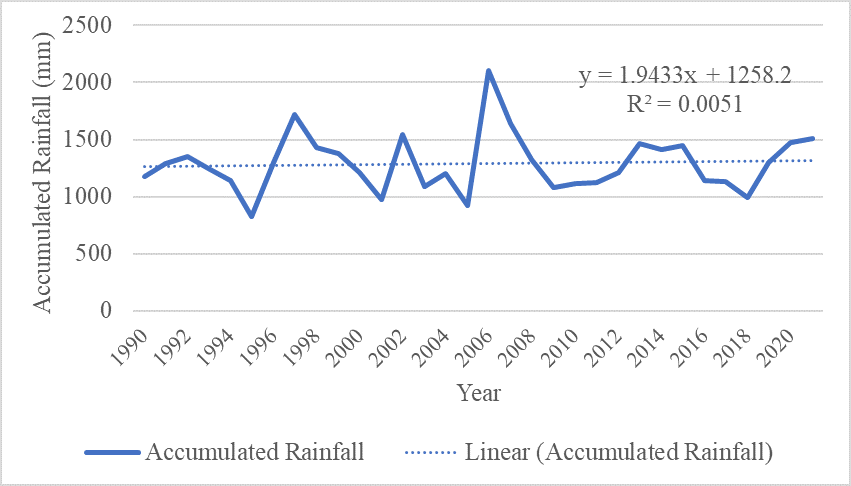
\includegraphics[width=0.9\textwidth]{images/trend_accumulated_rainfall.png}
\end{figure}


The graph~\ref{fig:trend_accumulated_rainfall} revealed a slight positive trend in accumulated rainfall $y=1.9433x + 1258.2$, with an annual increase of around 1.9433 millimeters per year. Changes in local weather patterns, air circulation, land use, and the effects of climate change might all be contributing factors to the increase in rainfall in Banke, Nepal.

\subsection{Correlation Between Yield and Climate Variables}


% Correlation Table
\begin{table}[htbp]
    \centering
    \caption{Correlation Table between Yield and Climate Variables}
    \resizebox{\textwidth}{!}{ % Resize table to fit within text width
    \begin{tabular}{@{}lccc@{}}
        \toprule
        & \textbf{Sunshine Hours} & \textbf{Accumulated Rainfall (mm)} & \textbf{Average Temperature (°C)} \\
        \midrule
        \textbf{Yield (mt/ha)} & 0.417* & -0.074 & 0.287 \\
        \textbf{(p-value)} & 0.017 & 0.686 & 0.112 \\
        \bottomrule
    \end{tabular}
    }
\end{table}

% Linear Regression Model Summary
\begin{table}[htbp]
    \centering
    \caption{Linear Regression Model Summary for Yield and Climate Data}
    \begin{tabular}{@{}lc@{}}
        \toprule
        \textbf{Dep. Variable} & Yield \\
        \textbf{Adjusted R-squared} & 0.161 \\
        \textbf{Significance (p-value)} & 0.048 \\
        \textbf{F-statistic} & 2.981 \\
        \textbf{R-squared} & 0.242 \\
        \bottomrule
    \end{tabular}
\end{table}

% Regression Coefficient Table
\begin{table}[htbp]
    \centering
    \caption{Regression Coefficients for Yield and Climate Data}
    \label{reg_coef_climate_yield}
    \resizebox{\textwidth}{!}{ % Resize table to fit within text width
    \begin{tabular}{@{}lccccll@{}}
        \toprule
        \multirow{2}{*}{\textbf{Model}} & \multicolumn{2}{c}{\textbf{Unstandardized Coefficients}} & \textbf{Standardized} & \multirow{2}{*}{\textbf{t}} & \multirow{2}{*}{\textbf{Sig}} \\
        \cmidrule{2-3}
        & \textbf{B} & \textbf{Std. Error} & \textbf{Beta} & & \\
        \midrule
        \textbf{(Constant)} & -99.061 & 903.331 & - & -0.110 & 0.913 \\
        \textbf{Sunshine} & 0.670 & 0.291 & 0.391 & 2.306 & 0.029 \\
        \textbf{Accumulated Rainfall} & -0.279 & 0.279 & -0.168 & -0.999 & 0.326 \\
        \textbf{Average Temperature} & 43.825 & 32.148 & 0.232 & 1.363 & 0.184 \\
        \bottomrule
    \end{tabular}
    }
\end{table}

\begin{equation}
    \begin{split}
        \text{Crop Yield} &= -99.061 + 0.670 \times \text{Sunshine} \\
        &\quad - 0.279 \times \text{Accumulated Rainfall} \\
        &\quad + 43.825 \times \text{Average Temperature}
    \end{split}
\end{equation}



Table 4.1 presents the correlation between crop yield and key climate variables, including sunshine hours, accumulated rainfall, and average temperature. The results indicate:

Sunshine hours show a significant positive correlation with yield (r = 0.417, p = 0.017), suggesting that increased solar exposure contributes to higher crop productivity.
Accumulated rainfall exhibits a weak negative correlation with yield (r = -0.074, p = 0.686), indicating that rainfall variability does not have a statistically significant effect on crop production.
Average temperature has a moderate positive correlation with yield (r = 0.287, p = 0.112), although the relationship is not statistically significant.
These findings suggest that sunshine hours play a more influential role in determining crop yield than rainfall or temperature variations.

Linear Regression Analysis
The linear regression model for yield and climate variables reveals an R-squared value of 0.242, indicating that approximately 24.2\% of the variability in crop yield can be explained by sunshine hours, accumulated rainfall, and average temperature. The adjusted R-squared value of 0.161 suggests a moderate explanatory power after adjusting for the number of predictors.

The regression model equation derived from the analysis is:


Regression Coefficients and Statistical Significance
Examining the individual regression coefficients:

Sunshine hours \(\beta = 0.391, \, p = 0.029\) show a significant positive effect on yield, confirming that increased sunlight exposure enhances productivity.
Accumulated rainfall \(\beta = -0.168, \, p = 0.326\) has a negative but non-significant effect, indicating that excessive or inconsistent rainfall does not significantly contribute to yield improvement.
Average temperature \(\beta = 0.232, \, p = 0.184\) has a positive but non-significant effect, suggesting that temperature variations alone are not a strong predictor of yield changes.
Discussion
Influence of Climate Factors on Crop Yield
The findings in Table \ref{reg_coef_climate_yield} indicate that sunshine hours are the most influential climate variable affecting crop yield. The significant positive correlation and regression coefficient confirm that higher solar radiation enhances photosynthesis, leading to better crop growth and productivity. This aligns with prior studies conducted in Nepal and South Asia, which found that solar radiation is a key determinant of agricultural output (Thapa \& Devkota, 2016).

Conversely, rainfall does not show a significant impact on yield, which may be due to erratic precipitation patterns in the Banke district. Similar studies in Nepal have reported that uneven rainfall distribution can reduce soil moisture availability, affecting crop health despite high total precipitation levels (Regmi et al., 2019). This suggests that rainfall variability, rather than total rainfall, may be more critical for crop yield determination.

The moderate but non-significant relationship between temperature and yield suggests that while temperature fluctuations impact crop growth, their effect is less direct than sunshine exposure. Previous research has found that higher temperatures may accelerate crop maturation but also increase evapotranspiration, reducing soil moisture levels and affecting plant growth (Shrestha et al., 2022). This could explain why the temperature variable, though positively correlated with yield, does not exhibit strong statistical significance.

Comparing with Previous Studies
Compared to previous studies in Nepal’s Terai region:

Devkota \& Paija (2020) found that a 1\% increase in rainfall improved rice yield by 0.45\%, while this study indicates a negative but weak relationship between rainfall and yield. The inconsistency may stem from differences in soil properties, irrigation availability, and crop types across districts.
Karki et al. (2021) reported that sunshine hours significantly influenced wheat productivity, supporting this study’s findings that higher solar exposure enhances crop output.
Risal et al. (2022) noted that temperature increases beyond optimal thresholds negatively impact yield, whereas this study does not find a strong negative effect, possibly due to regional climate adaptations.
Implications for Agricultural Adaptation Strategies
The results underscore the importance of optimizing sunshine exposure through improved crop management techniques such as:
Selecting drought-resistant crop varieties that can capitalize on high sunlight conditions.
Enhancing irrigation infrastructure to mitigate the negative impacts of inconsistent rainfall.
Adopting precision agriculture technologies to optimize planting schedules based on temperature and solar radiation patterns.

Additionally, policymakers should focus on climate-resilient agricultural practices, particularly in districts like Banke, where rainfall unpredictability poses challenges for farmers.

Limitations \& Future Research Directions
Although this study provides valuable insights, some limitations should be considered:

The relatively low R-squared value (0.242) suggests that other non-climatic factors (e.g., soil quality, pest outbreaks, irrigation methods) also influence yield and should be included in future models.
The study does not account for extreme weather events (e.g., floods, droughts), which could significantly affect yield trends.
Future research should incorporate long-term climate projections and soil moisture analysis to improve yield prediction accuracy.
Conclusion
This study highlights the strong positive impact of sunshine hours on crop yield, while rainfall and temperature have weaker, non-significant effects. The findings suggest that improving water management and leveraging sunshine exposure are key to sustaining agricultural productivity in Nepal’s Banke district. Future studies should integrate broader climate and agronomic factors to develop more comprehensive yield forecasting models.


subsubsection{Climate Change Perception}

Table~\ref{tab:farmer_perception} shows the farmers' perception towards questions related to climate change. The results indicate that all the farmers in the study area were aware of the ongoing general climate change, with an index value of 1. However, there was almost no awareness about the range of temperature experienced in the locality and its effects on agricultural productivity, both having an index value of -0.88. 

Farmers were highly unaware of the effects of climate change regarding untimely monsoons and their impact on production, with an index value of -0.75. On the other hand, farmers had slight awareness about the effects of pests and insects, abnormalities in crops due to climate change, and extreme weather events in the locality, with index values of 0.28, 0.275, and 0.155, respectively. 

Even though all farmers were aware of the ongoing climate change, there was only an average level of awareness about the evidence of climate change. The detailed calculations are presented in Annex 5.

\begin{table}[htbp]
    \centering
    \caption{Farmer’s Perception on Climate Data}
    \label{tab:farmer_perception}
    \begin{tabular}{@{}lcc@{}}
        \toprule
        \textbf{Statement / Variables} & \textbf{Index} \\
        \midrule
        Climate change is happening & 1.00 \\
        Aware about the range of temperature experienced in locality & -0.88 \\
        Climate change affects agricultural productivity & -0.88 \\
        Effect of untimely monsoon on production & -0.75 \\
        Climate change affects the spread of pests and insects over crops & 0.28 \\
        Abnormalities in crops & 0.275 \\
        Extreme events in locality & 0.155 \\
        Evidence of climate change & 0.47 \\
        \bottomrule
    \end{tabular}
    \vspace{0.5cm}

    \textit{*Higher the index, stronger the perception.} \\
    \textit{Frequency of agreement/approval: +1, Frequency of disagreement/disapproval: -1, Frequency of don't know/absent: 0.}
\end{table}

\subsubsection{agriculture and Food Scenarios}
Table~\ref{tab:agriculture_food_scenario} presents the production-related data obtained from the household survey conducted in the study area. The findings indicate that mixed farming and crop combination were almost nonexistent, with 97.8\% of households not practicing either method. 

The study further revealed that 92.5\% of families produced enough food for themselves, while 3\% of families met their food deficit by purchasing from the market. Despite the minimal institutional support, recorded at only 4.5\%, a significant portion (97.8\%) of the population had sufficient food stock. This was primarily sourced from their own production (95.5\%), with the remaining 4.5\% obtained from markets. 

As a result, the majority of the population (99.3\%) was well-nourished, with only 0.7\% identified as undernourished (Annex 6.7).

\begin{table}[htbp]
    \centering
    \caption{Agricultural and Food Scenario Characteristics}
    \label{tab:agriculture_food_scenario}
    \begin{tabular}{@{}lcc@{}}
        \toprule
        \textbf{Characteristics} & \textbf{Variables} & \textbf{Percentage} \\
        \midrule
        Mixed Farming & Yes & 2.2 \\
                     & No & 97.8 \\
        Crop Combination & Yes & 2.2 \\
                         & No & 97.8 \\
        Food Production & Enough & 92.5 \\
                        & Not Enough & 7.5 \\
        Food Deficit & Purchase from the market & 3.0 \\
                     & Not Deficit & 97.0 \\
        Undernutrition & No & 99.3 \\
                       & Yes & 0.7 \\
        Food Stock Present or Absent & Yes, Present & 97.8 \\
                                     & No, Absent & 2.2 \\
        Sources & Own Production & 95.5 \\
                & Markets & 4.5 \\
        Institutional Support & Yes & 4.5 \\
                              & No & 95.5 \\
        \bottomrule
    \end{tabular}
\end{table}

subsubsection{Crop Calendar}
Farmers in the study area have shifted their sowing and harvesting times over the past five years (Table~\ref{tab:crop_calendar}). The primary reason behind this shift in cropping time is attributed to irregular monsoons and climatic changes. However, for seasonal fruits and vegetables, no significant changes were observed. 

\begin{table}[htbp]
\centering
\caption{Crop Calendar Based on Major Changes in Cropping Time}
\label{tab:crop_calendar}
\resizebox{\textwidth}{!}{  
    \begin{tabular}{@{}lccccc@{}}
        \toprule

        \textbf{Crop} & \multicolumn{2}{c}{\textbf{Before 5 Years}} & \multicolumn{2}{c}{\textbf{Recent Time (After 5 Years)}} & \textbf{Reason} \\
        \cmidrule(lr){2-3} \cmidrule(lr){4-5}
        & \textbf{Sowing Month} & \textbf{Harvesting Month} & \textbf{Sowing Month} & \textbf{Harvesting Month} &  \\

        \hline
        Paddy & June (3rd week) & September (1st week) & August (1st week) & November (Mid-week) & Irregular Monsoon / Climatic Shift \\
        Wheat & December (1st week) & April (Last week) & January (Mid-week) & April (2nd week) & Climatic Shift \\
        Mustard & November (Mid-week) & April (Mid-week) & November (3rd week) & March (2nd week) & Climatic Shift \\
        Lentils & October (3rd week) & March (3rd week) & December (1st week) & April (Last week) & Climatic Shift \\
        Pigeon Pea & June (Last week) & January (2nd week) & July (3rd week) & February (2nd week) & Climatic Shift \\
        Vegetables & All months & All months & All months & All months & No Change \\
        Fruits & All months & All months & All months & All months & No Change \\
        \hline
    \end{tabular}
}
    \vspace{0.5cm}

    \textit{Source: Questionnaire survey conducted in the study area.}
\end{table}

\subsection{Irrigation}
\subsubsection{irrigation Status}
Numerous irrigation sources are used in the research region. During the monsoon season, 93.3\% of the land relies on rainfed irrigation, while only 26.9\% of the land has irrigation available throughout the year. The entire study area is covered by gravity-fed surface irrigation, which includes both flood and furrow techniques. Additionally, respondents reported that there were no significant issues related to irrigation in the study area (Table~\ref{tab:irrigation_data}).

\begin{table}[htbp]
    \centering
    \caption{Frequency Table for Land and Irrigation Data of Survey}
    \label{tab:irrigation_data}
    \begin{tabular}{@{}lcc@{}}
        \toprule
        \textbf{Characteristics} & \textbf{Variables} & \textbf{Percentage} \\
        \midrule
        \multirow{4}{*}{Irrigation Source} & Ground water + Canal irrigation + Rainfall & 23.9 \\
        & Ground water + Drainage Pond + Rainfall & 59.0 \\
        & Ground water + Rainfall & 1.5 \\
        & All & 15.7 \\
        \midrule
        \multirow{2}{*}{Land Quality Irrigation} & Khet & 73.1 \\
        & Upland and Khet & 26.9 \\
        \midrule
        \multirow{3}{*}{Irrigation Type} & Natural & 38.1 \\
        & Artificial & 48.5 \\
        & Both & 13.4 \\
        \midrule
        \multirow{2}{*}{Irrigation Category} & Year-round irrigation (whole year) & 6.7 \\
        & Rainfed Irrigation (monsoon) & 93.3 \\
        \midrule
        \multirow{2}{*}{Season of Availability} & All Season & 26.9 \\
        & Monsoon & 73.1 \\
        \midrule
        Irrigation Technique & Gravity-fed surface (flood and furrow) & 100.0 \\
        \bottomrule
    \end{tabular}
\end{table}

\subsubsection{Irrigation and yield}


The different categories of irrigation used in the study area were categorized into two irrigation groups: year-round irrigation, used by 9 respondents, and rainfed irrigation, used by 125 respondents (Annex 6.3). Table~\ref{tab:t_test_irrigation} presents the results of the t-test examining the effect of different irrigation categories on crop yield.

\begin{table}[htbp]
    \centering
    \caption{t-test of Between-Subjects Effects}
    \label{tab:t_test_irrigation}
    \begin{tabular}{@{}l c c c c c c@{}}
        \toprule
        & \multicolumn{2}{c}{\textbf{Year-Round Irrigation}} & \multicolumn{2}{c}{\textbf{Rainfed Irrigation}} & \multicolumn{2}{c}{t(132), p} \\
        \cmidrule(lr){2-3} \cmidrule(lr){4-5}
        \textbf{Yield (kg/ha)} & \textbf{Mean} & \textbf{SD} & \textbf{Mean} & \textbf{SD} & \textbf{t} & \textbf{p} \\
        \midrule
        Crop Yield & 7868.63 & 3756.38 & 5450.43 & 2505.86 & 2.696 & 0.008 \\
        \bottomrule
    \end{tabular}
\end{table}

The t-test results compare the mean yield between two irrigation methods, year-round irrigation and rainfed irrigation, in Janaki Rural Municipality (Table~\ref{tab:t_test_irrigation}). The findings indicate that for year-round irrigation, the mean yield is 7868.63 kg/ha with a standard deviation of 3756.38, while for rainfed irrigation, the mean yield is 5450.43 kg/ha with a standard deviation of 2505.86. 

The higher crop yield in year-round irrigation can be attributed to the fact that individual household crop yields were computed separately and then aggregated to determine the overall yield. The analysis revealed a statistically significant difference in mean yields between the two groups, \( t(132) = 2.696, p = 0.008 \), suggesting that year-round irrigation significantly enhances crop yield compared to rainfed irrigation.


